\documentclass[11pt]{article}%
\usepackage[T1]{fontenc}%
\usepackage[utf8]{inputenc}%
\usepackage{lmodern}%
\usepackage{textcomp}%
\usepackage{lastpage}%
%
\usepackage[table]{xcolor}%
\usepackage{setspace}%
\usepackage{graphicx}%
\usepackage{tikz}%
\usepackage{atbegshi,picture}%
\usepackage[a4paper, total={7in, 10.5in}]{geometry}%
\usepackage{siunitx}%
\usepackage{fixltx2e}%
\usepackage[pscoord]{eso-pic}%
\renewcommand{\familydefault}{\sfdefault}%
\newcommand{\placetextbox}[3]{\setbox0=\hbox{#3}\AddToShipoutPictureFG*{\put(\LenToUnit{#1\paperwidth},\LenToUnit{#2\paperheight}){\vtop{{\null}\makebox[0pt][c]{#3}}}}}%
\setlength{\arrayrulewidth}{0.2pt}%
\setlength{\tabcolsep}{8pt}%
\renewcommand{\arraystretch}{1.9}%
\arrayrulecolor[HTML]{999999}%
\AtBeginShipoutNext{\AtBeginShipoutUpperLeft{\put(\dimexpr\paperwidth-1.5cm\relax,-2.42cm){\makebox[0pt][r]{\Large Empowering Laser Technologies}}}}%
%
\begin{document}%
\normalsize%
\begin{tikzpicture}[remember picture,overlay]\node[anchor=north west,yshift=-25.0pt,xshift=40pt] at (current page.north west){
\includegraphics[height=1.5cm]{pics/logo.pdf}};\end{tikzpicture}%
\vspace{22mm}%
\begin{spacing}{1.5}%
\begin{center} {\huge \textbf{Test Data Sheet} \par}%
\end{center}%
\end{spacing}%
\begin{center} {\Large\textbf{PM7-SWIR1\_20} \par} \end{center}%
\begin{center} {\normalsize 22.1235 \par} \end{center}%
\begin{center} {\Large \textbf{Resonant electro-optic phase modulator}}\end{center}%
\begin{figure}[h]%
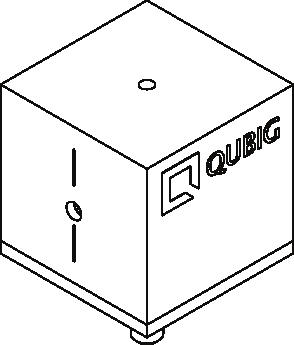
\includegraphics[width=4cm]{pics/Cube_page1}%
\centering%
\end{figure}%
\begin{table}[h]%
\centering%
\begin{tabular}{ |p{9.5cm}|p{3cm}|p{2.0cm}|  }%
\hline%
\rowcolor[HTML]{153c4a}%
\textcolor{white}{\textbf{RF properties}}  & \hfil \textcolor{white}{\textbf{Value}} & \hfil \textcolor{white}{\textbf{Unit}}  \\%
\hline%
Resonance frequency: f$_{0}$ $^{1)}$   & \hfil 5.0 & \hfil MHz \\%
\hline%
Bandwidth: $\Delta \nu$  & \hfil 101   & \hfil kHz \\%
\hline%
Quality Factor: Q & \multicolumn{2}{|c|}{8}  \\%
\hline%
Required RF power for 1rad $@$ 852nm $^{2)}$   & \hfil 9.3 & \hfil dBm \\%
\hline%
max. RF power: RF\textsubscript{max} $^{3)}$ & \hfil 0.5   & \hfil W \\%
\hline%
\end{tabular}%
\end{table}%
\vspace{-5mm}%
\begin{table}[h]%
\centering%
\begin{tabular}{ |p{9.5cm}|p{3cm}|p{2.0cm}|  }%
\hline%
\rowcolor[HTML]{153c4a}%
\textcolor{white}{\textbf{Optical properties}}  & \hfil \textcolor{white}{\textbf{Value}} & \hfil \textcolor{white}{\textbf{Unit}} \\%
\hline%
Aperture & \hfil 3x3 & \hfil mm$^2$ \\%
\hline%
Wavefront distortion (633nm) & \hfil $\lambda / 6$   & \hfil nm \\%
\hline%
Recommended optical intensity (852nm) & \hfil \si{<} 1 & \hfil W/mm$^2$ \\%
\hline%
AR coating (R\textsubscript{avg}\si{<}1\% ) & \hfil 630 - 1100 & \hfil nm  \\%
\hline%
\end{tabular}%
\end{table}%
\placetextbox{0.30}{0.06}{\scriptsize $^{1)}$25°C   $^{2)}$with 50$\si{\ohm}$ termination   $^{3)}$no damage with RF\textsubscript{in}\si{<}1W  }%
%
%
%
%
\end{document}